\documentclass{beamer}

\usetheme{Madrid}
\usecolortheme{default}

\usepackage{amsmath, amssymb}
\usepackage{physics}
\usepackage{tikz}
\usepackage{siunitx}
\usepackage{tcolorbox}

\title[Physics 122]{Physics 122 \\ Thermal Physics}
\author{Lecture Notes}
\date{}

\begin{document}

%------------------------------------------------
\begin{frame}
  \titlepage
\end{frame}

%------------------------------------------------
\begin{frame}{Outline}
\tableofcontents
\end{frame}

%------------------------------------------------
\section{Adiabatic Processes}

\begin{frame}{What is an Adiabatic Process?}
\begin{tcolorbox}
An \textbf{adiabatic process} is a thermodynamic process in which
\[
\boxed{Q = 0}
\]
(no heat exchange with the surroundings).
\end{tcolorbox}

\pause
\textbf{Occurs when:}
\begin{itemize}
  \item Process is very fast
  \item System is thermally insulated
\end{itemize}
\end{frame}

%------------------------------------------------
\begin{frame}{First Law of Thermodynamics}
\begin{tcolorbox}
\textbf{Physics 122 sign convention:}

Work done \emph{by the environment on the system} is positive.
\end{tcolorbox}

\[
\boxed{\Delta E = Q + W}
\]

\pause
For an adiabatic process:
\[
\boxed{\Delta E = W}
\]
\end{frame}

%------------------------------------------------
\begin{frame}{Physical Interpretation}
\begin{itemize}
  \item \textbf{Compression:}
  \[
  W>0 \Rightarrow \Delta E>0 \Rightarrow T \uparrow
  \]
  \pause
  \item \textbf{Expansion:}
  \[
  W<0 \Rightarrow \Delta E<0 \Rightarrow T \downarrow
  \]
\end{itemize}

\pause
\textbf{Examples:}
\begin{itemize}
  \item Diesel engine compression
  \item Opening a soda bottle
  \item Spraying deodorant
\end{itemize}
\end{frame}

%------------------------------------------------
\section{Adiabatic vs Isothermal}

\begin{frame}{Ideal Gas Processes}
\[
PV = nRT
\]

\pause
\textbf{Isothermal:}
\[
T = \text{constant}, \quad P = \frac{nRT}{V}
\]

\pause
\textbf{Adiabatic:}
\[
\boxed{PV^\gamma = \text{constant}}
\quad
\gamma = \frac{C_P}{C_V}
\]
\end{frame}

%------------------------------------------------
\begin{frame}{P--V Diagram}
\begin{center}
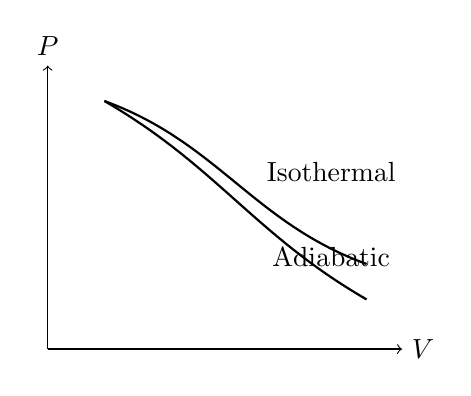
\begin{tikzpicture}[scale=0.9]
  \draw[->] (0,0) -- (5,0) node[right] {$V$};
  \draw[->] (0,0) -- (0,4) node[above] {$P$};

  \draw[thick] (0.8,3.5) to[out=-20,in=160] (4.5,1.2);
  \node at (4,2.5) {Isothermal};

  \draw[thick] (0.8,3.5) to[out=-30,in=150] (4.5,0.7);
  \node at (4,1.3) {Adiabatic};
\end{tikzpicture}
\end{center}

\pause
\textbf{Adiabatic curves are steeper.}
\end{frame}

%------------------------------------------------
\section{Thermal Expansion}

\begin{frame}{Linear Expansion}
\begin{tcolorbox}
\[
\boxed{\Delta L = \alpha L_0 \Delta T}
\]
\end{tcolorbox}

\pause
\begin{itemize}
  \item $\alpha$ = coefficient of linear expansion
  \item Units: \(\si{K^{-1}}\)
  \item Depends on material
\end{itemize}
\end{frame}

%------------------------------------------------
\begin{frame}{Volume Expansion}
\[
\boxed{\Delta V = \beta V_0 \Delta T}
\]

\pause
For isotropic solids:
\[
\boxed{\beta \approx 3\alpha}
\]
\end{frame}

%------------------------------------------------
\begin{frame}{Microscopic Picture}
\begin{center}
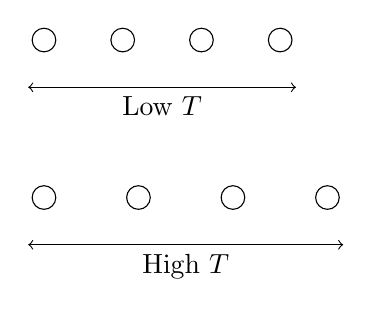
\begin{tikzpicture}
  \foreach \x in {0,1,2,3} {
    \draw (\x,0) circle (0.15);
  }
  \draw[<->] (-0.2,-0.6) -- (3.2,-0.6) node[midway,below] {Low $T$};

  \foreach \x in {0,1.2,2.4,3.6} {
    \draw (\x,-2) circle (0.15);
  }
  \draw[<->] (-0.2,-2.6) -- (3.8,-2.6) node[midway,below] {High $T$};
\end{tikzpicture}
\end{center}

\pause
Higher temperature $\Rightarrow$ larger atomic vibrations $\Rightarrow$ expansion.
\end{frame}

%------------------------------------------------
\section{Worked Example}

\begin{frame}{Linear Expansion Example}
\textbf{Given:}
\[
L_0 = \SI{10}{m}, \quad \alpha = 12\times10^{-6}\,\si{K^{-1}}
\]
\[
\Delta T = 40^\circ\text{C}
\]

\pause
\textbf{Solution:}
\[
\Delta L = \alpha L_0 \Delta T
\]
\[
\boxed{\Delta L = 4.8\,\text{mm}}
\]
\end{frame}

%------------------------------------------------
\begin{frame}{Key Takeaways}
\begin{itemize}
  \item Adiabatic process: \(Q=0\)
  \item Physics 122 convention: \(\Delta E = Q + W\)
  \item Compression heats, expansion cools
  \item Thermal expansion scales with \(\Delta T\)
\end{itemize}
\end{frame}

\end{document}
